% Use xelatex to generate pdf file of this presentation

\documentclass{beamer}
\usepackage{roboto}
\usepackage[russian]{babel}
\usetheme{Copenhagen}

% Simple way to put a code listing to the slide
\usepackage{listings}

\usepackage{tikz}
\usepackage{graphicx}
  \logo{
\includegraphics[scale=0.1]{PostgresPro_logo}}
%Information to be included in the title page:
\title{Query plan freezing extension}
\subtitle{design,\ issues\ and\ lessons\ learned}
\author{Belyalov D., \underline{Lepikhov A.}, Rybakina A.}
\institute{Postgres Professional}
%\titlegraphic{\includegraphics[scale=0.05]{project_url}}
\date{2023}

% Add page numbers in footnote
\expandafter\def\expandafter\insertshorttitle\expandafter{%
  \insertshorttitle\hfill%
  \insertframenumber\,/\,\inserttotalframenumber}

\definecolor{lightlightgray}{gray}{0.9}

% -----------------------------

\begin{document}

\begin{frame}
\titlepage
   \tikz [remember picture,overlay]
    \node at
        ([yshift=2.0cm, xshift=-4.2cm]current page.center) 
        {
\includegraphics[scale=0.034]{project_logo}};
\end{frame}

\begin{frame}[fragile]\frametitle{Self Introduction}
\begin{itemize}
  \item Specialist in Applied Mathematics graduated from Chelyabinsk State University in 2005
  \item Ph.D. in Computer Sciences (Distributed Databases) awarded at Moscow State University in 2008.
  \item Working in Postgres Professional as a Core Developer since 2017.
  \item Designed the Shardman project architecture on its earlier steps
  \item Worked on Multimaster project
  \item Working on various query optimization issues
\end{itemize}
\end{frame}

\begin{frame}[fragile]\frametitle{Who we are}
\begin{itemize}
  \item Research team, part of Postgres Professional, dealing with optimization issues
  \item Caused by the idea of sustainable coding
  \item Design enterprise and core features to improve the planner effectiveness
  \item Projects: Self-Join Removal, Asymmetric JOIN, Optimized Group-by, AQO, sr\_plan ...

% Some of our projects you could already know, reading hackers mailing list or using PGPRO products, but some of the products, like replanning or adaptive join is still under development.
% But general idea still the same: create effective plans and provide a set of tools to manually correct mistakes if optimizer has failed.
\end{itemize}
\end{frame}

\begin{frame}[fragile]\frametitle{Plan freezing?}
\begin{columns}\begin{column}{0.6\textwidth}
\textbf{Reason 1:} \\
Don't optimize next time! \\
%\vspace{5mm}
\bigskip
pgbench:
\begin{itemize}
  \item With planning: $\approx$ 3300 tps
  \item Prepared statements: $\approx$ 4300 tps
\end{itemize}
% pgbench with prepared queries and not - reveals the potential
\end{column}
\begin{column}{0.4\textwidth}
  
\includegraphics[scale=0.7]{chalkboardlines}
\end{column}\end{columns}
\end{frame}

\begin{frame}[fragile]\frametitle{Plan freezing?}
\begin{columns}\begin{column}{0.6\textwidth}
\textbf{Reason 2:} \\
Pin tweaked query plan into the plan cache:
\begin{itemize}
  \item Predictable execution time
  \item No planning surprises after minor upgrade
\end{itemize}
\end{column}
\begin{column}{0.4\textwidth}
  \begin{center}
    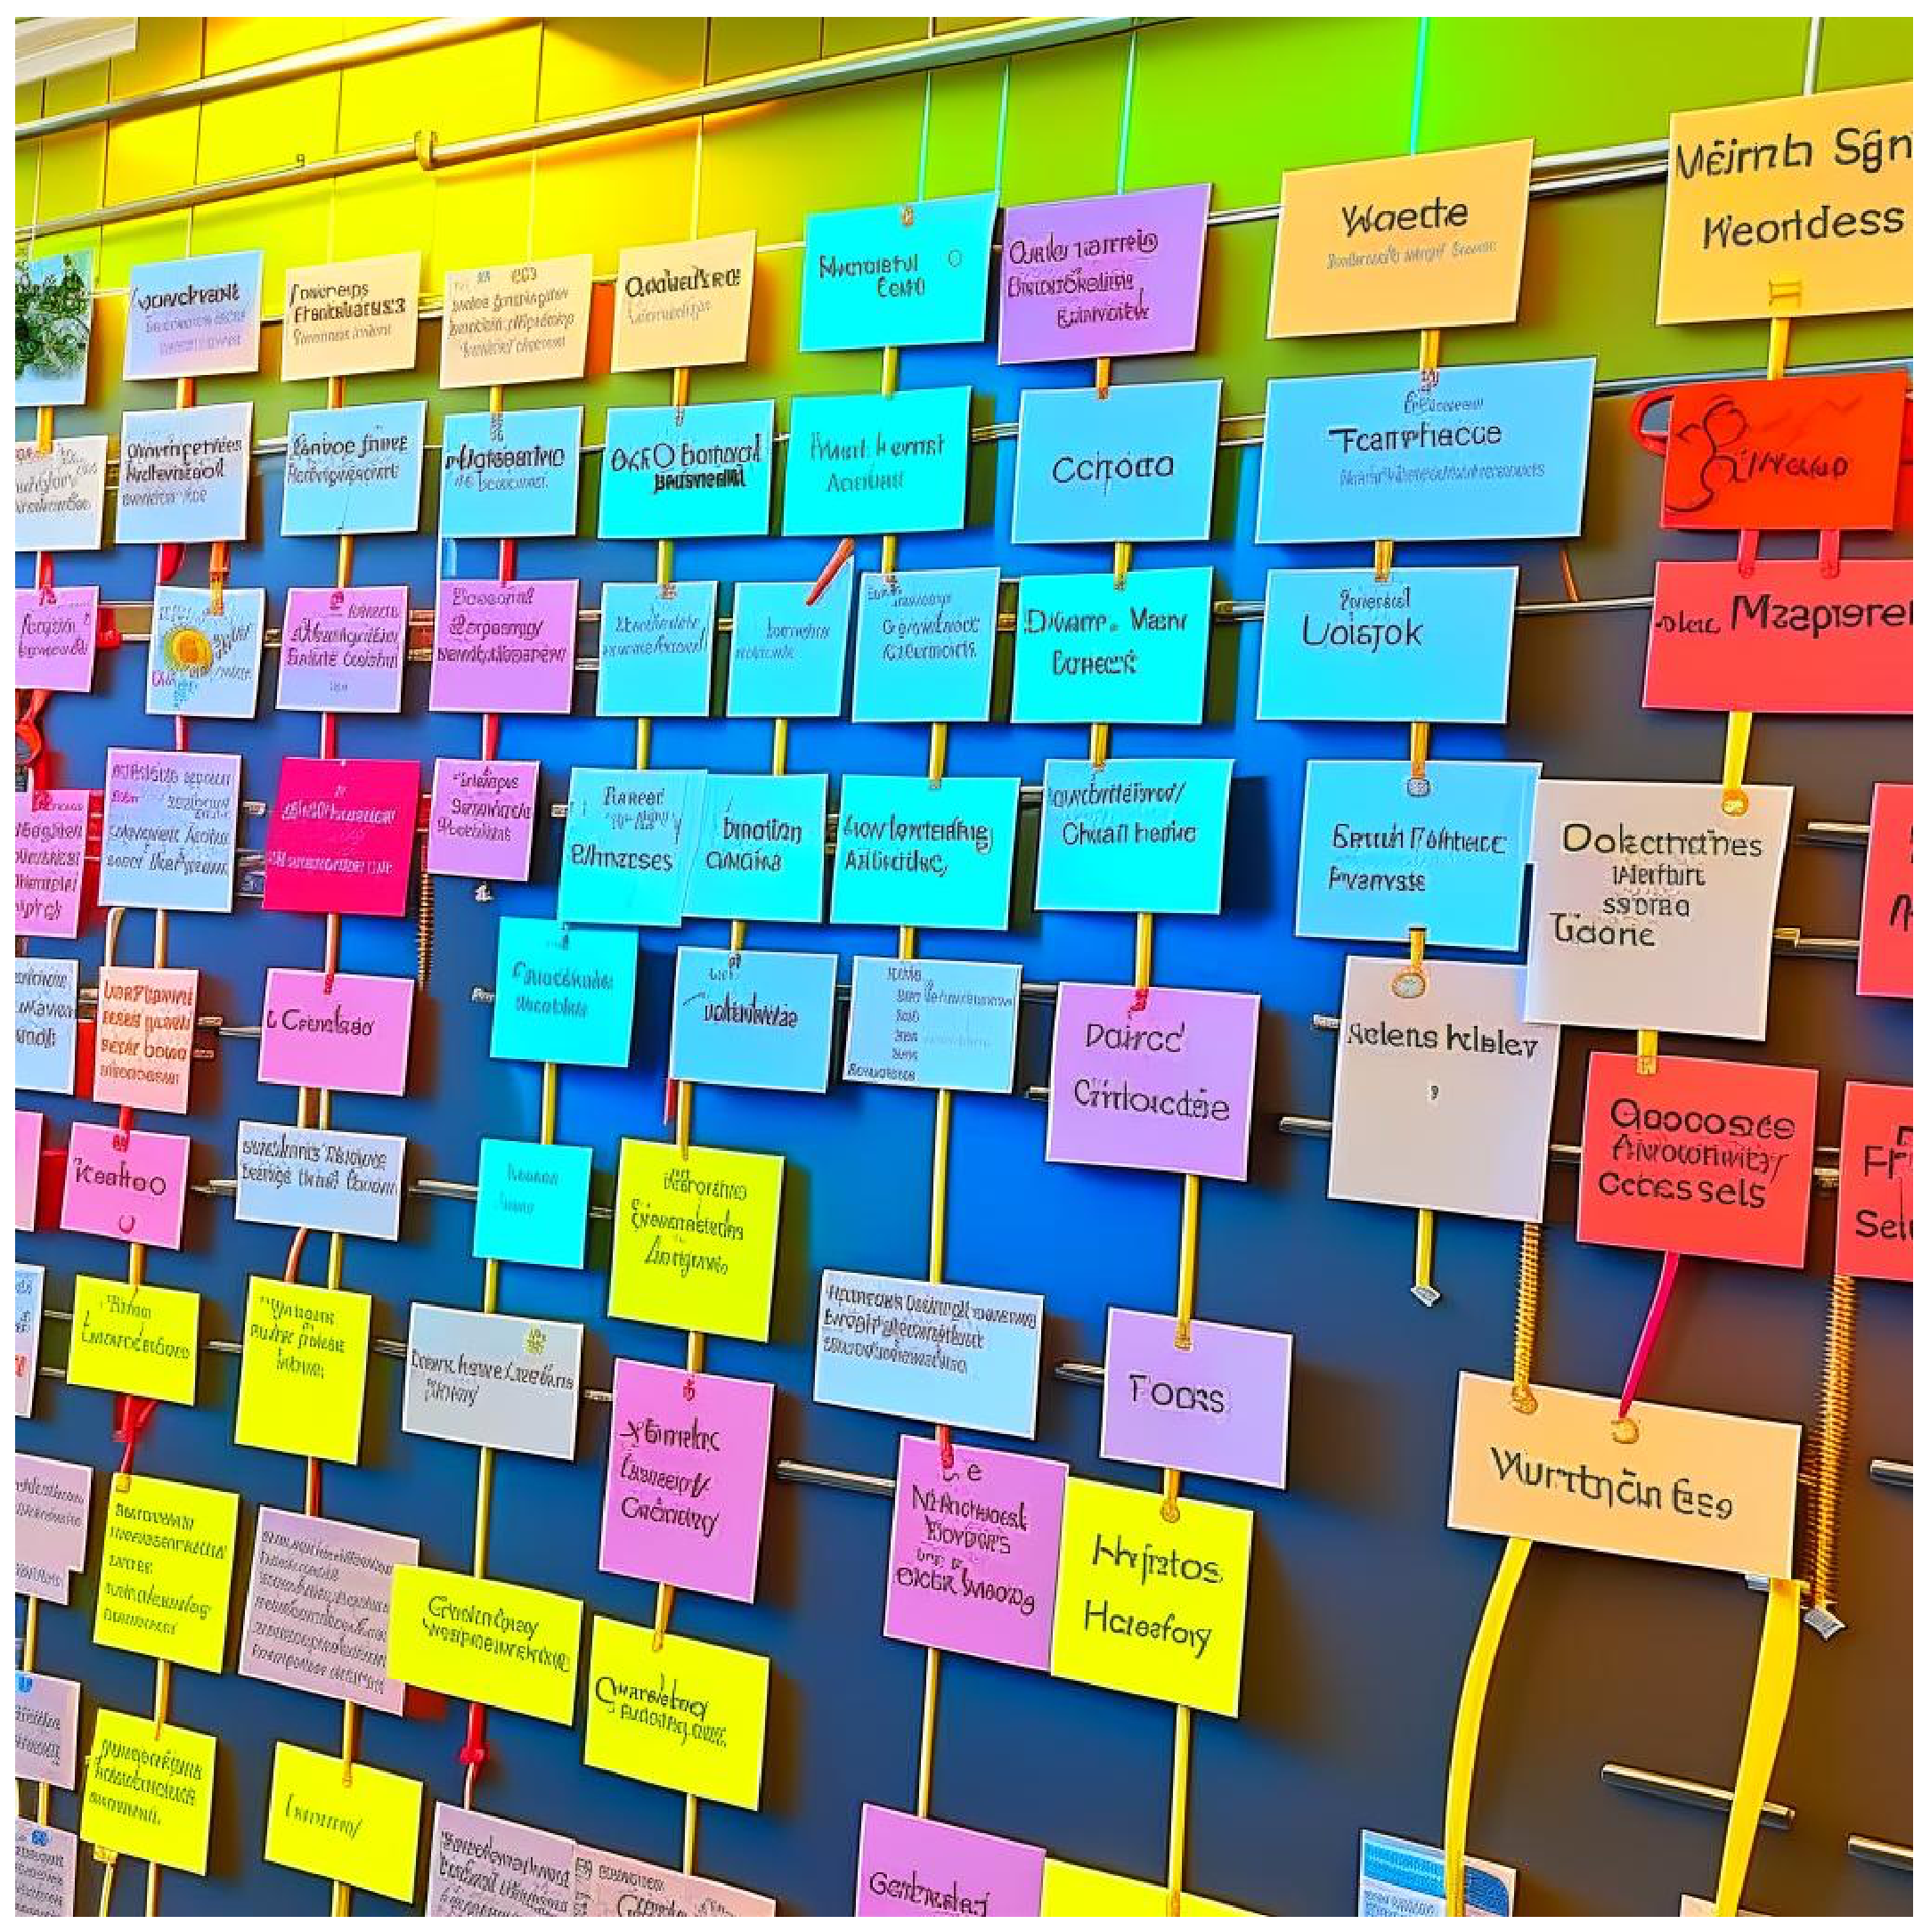
\includegraphics[scale=0.1]{stickers}
  \end{center}
\end{column}\end{columns}
\end{frame}

\begin{frame}[fragile]\frametitle{Rationale}
% What is the origins of the idea to freeze plans
\begin{itemize}
  \item Stale statistics
  \item Imperfection of cost estimation algorithms
  \item Implicit functional dependencies between columns
% No one wants to do vacuum frequently. If you have queries which is quite complex, containing composite scan clauses and extract some small set of data from big tables, you should have actual statistics. Another way you have a risk to end up with non-optimal query plans. Query plan freezing here is a hack to delay vacuum or, at least, don't stuck into the problem unexpectedly.
% Second issue related to bugs, changes in cost model during pg_upgrade and other problems with the cost model we all know.
% And the most frequent last issue related to hidden functional dependencies. In practice it is the most awkward problem: we spend a lot of time to handle non-optimal plans here but at most can't do anything because PostgreSQL couldn't have tools to resolve it in common case.
% To briefly explain this issue, I want to show two cases.
\end{itemize}
\end{frame}

\begin{frame}[fragile]\frametitle{Functional Dependencies (overestimation)}
\lstset{language=sql, frame=none, tabsize=2, identifierstyle=\color{black},
  backgroundcolor=\color{lightlightgray},
  keywordstyle=\bfseries\color{green!40!black},showspaces=false, showtabs=false, showstringspaces=false}
\begin{lstlisting}[basicstyle=\footnotesize]
CREATE TABLE people (
  name          text,
  occupation    text,
  sex           boolean,
  region        text,
  is_vaccinated boolean
);
\end{lstlisting}
\begin{lstlisting}[basicstyle=\footnotesize]
SELECT * FROM people t1
WHERE occupation = 'Tractor Driver' AND sex = 'female'
/*
Seq Scan on people  (rows=1584) (actual rows=1)
   Filter: (is_woman AND (occupation = 'Tractor Driver'))
   Rows Removed by Filter: 99999
 */
\end{lstlisting}
\end{frame}

\begin{frame}[fragile]\frametitle{Functional Dependencies (underestimation)}
\lstset{language=sql, frame=none, tabsize=2, identifierstyle=\color{black},
  backgroundcolor=\color{lightlightgray},
  keywordstyle=\bfseries\color{green!40!black},showspaces=false, showtabs=false, showstringspaces=false}
\begin{lstlisting}[basicstyle=\footnotesize]
CREATE TABLE people (
  name          text,
  occupation    text,
  sex           boolean,
  region        text,
  is_vaccinated boolean
);
\end{lstlisting}
\begin{lstlisting}[basicstyle=\footnotesize]
SELECT * FROM people
WHERE region = 'Chelyabinsk' AND is_vaccinated;
/*
 Seq Scan on people  (rows=114) (actual rows=907)
   Filter: (is_vaccinated AND (region = 'Chelyabinsk'))
   Rows Removed by Filter: 99094
 */
\end{lstlisting}
\end{frame}

% Here we need some bridge from the planner slip-ups to the plan freezing
\begin{frame}[fragile]\frametitle{Our conjecture}
\begin{quote}
Unfortunate planning is inevitable [at least, for now]. Assuming someone or something could force the planner to generate a better plan, we should provide the tool to freeze the right solution for the subsequent executions.
\end{quote}
\end{frame}

\begin{frame}[fragile]\frametitle{Stick on the plan in the Plan Cache ?}
\begin{center}
  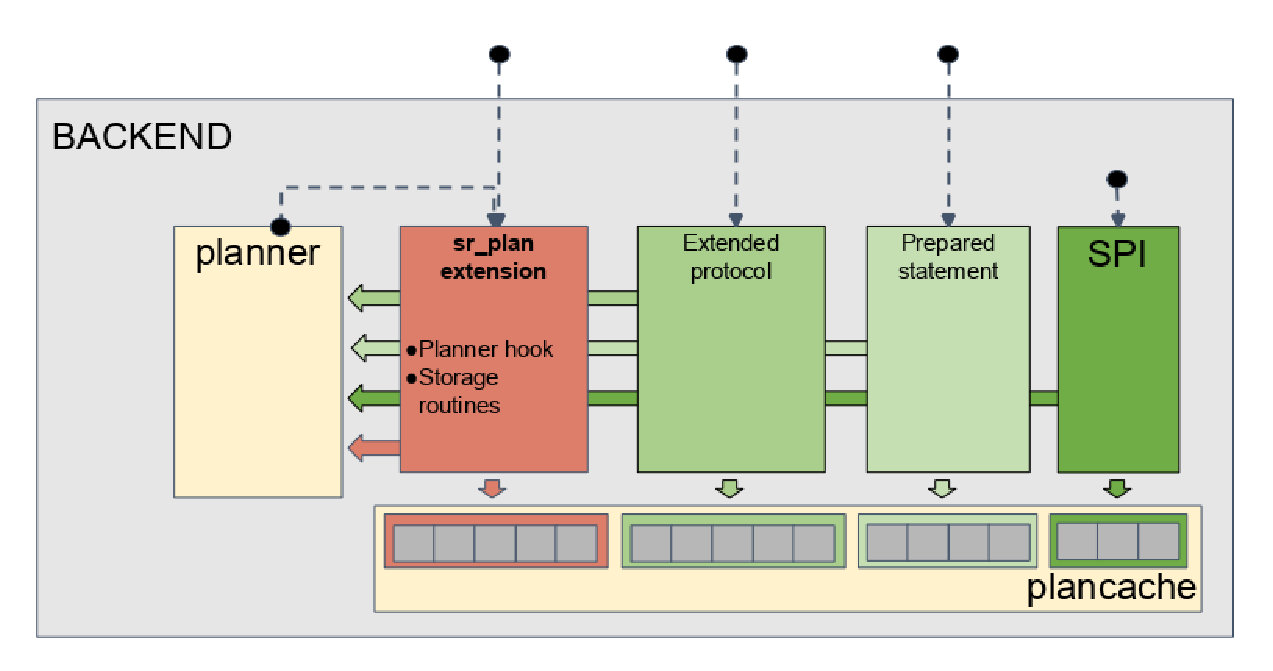
\includegraphics[width=\textwidth]{plancache_callers}
\end{center}
%\begin{itemize}
%  \item PostgreSQL already have local plan cache in each backend
%  \item Prepared Statements use it
%  \item Extended Query Protocol uses it
%  \item Stored procedures can use it
%\end{itemize}
% So, what we really need to do is to implement global prepared statements.
\end{frame}

\begin{frame}[fragile]\frametitle{The sr\_plan extension}
\begin{columns}\begin{column}{0.8\textwidth}
\begin{itemize}
  \item Abbreviates \textbf{s}ave/\textbf{r}estore plan 
  \item Introduced in Postgres Pro Enterprise 15 (don\'t mix up with the extension sr\_plan existed up to PGPro Enterprise 13!)
  \item Freezes specific plan for a [parameterized] query
  % https://postgrespro.com/docs/enterprise/15/sr-plan
\end{itemize}
\end{column}
\begin{column}{0.2\textwidth}
  
\includegraphics[scale=0.7]{srplanqr}
\end{column}
\end{columns}
\end{frame}

\begin{frame}[fragile]\frametitle{How it works}
\begin{itemize}
  \item sr\_register\_query('SELECT ... WHERE x = \$1 AND y = 42', ...)
  \item sr\_plan\_freeze(srid)
  \item sr\_plan\_unfreeze(srid)
\end{itemize}
\begin{block}{Frozen plan have a special node in explain}
\begin{lstlisting}[basicstyle=\footnotesize]
                            QUERY PLAN          ------------------------------------------------
 Custom Scan (SRScan) (actual rows=1 loops=1)
   Frozen plan ID: 1
   ->  Aggregate (actual rows=1 loops=1)
      ->  Seq Scan on a (actual rows=10 loops=1)
            Filter: ((x = \$1) AND (y = 42)
\end{lstlisting}\end{block}
\end{frame}

\begin{frame}[fragile]\frametitle{Lesson 1}
\begin{columns}\begin{column}{0.5\textwidth}
In DBMS, the way from a query text to the plan is not straightforward.
\end{column}\begin{column}{0.5\textwidth}
\begin{center}
  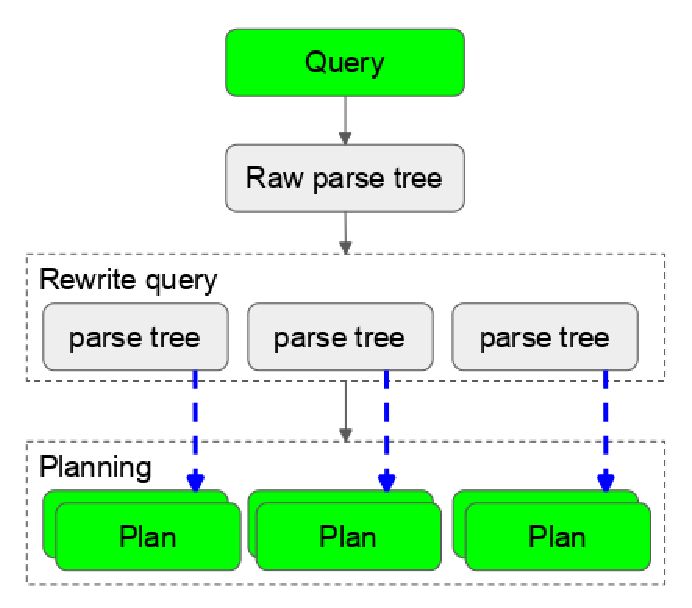
\includegraphics[scale=0.5]{query_planning_stages}
% It is not enough to save somewhere the query text to provable use frozen plan we saved earlier. Because rewriting rules can be changed. Moreover, backspaces and other cosmetic changes of the query which don't change its semantic will cause using of non-frozen plan.
% It is not enough even to store raw parse tree and prove usability of the plan by the equality of stored and incoming tree. Only one way to prove usability of the plan for the given query is to compare stored and incoming parse trees.
\end{center}\end{column}\end{columns}
\end{frame}

\begin{frame}[fragile]\frametitle{Lesson 2}
\begin{columns}\begin{column}{0.5\textwidth}
Only one way to prove applicability of the plan to the given query is to compare stored and incoming parse trees
\end{column}\begin{column}{0.5\textwidth}
  \begin{center}
    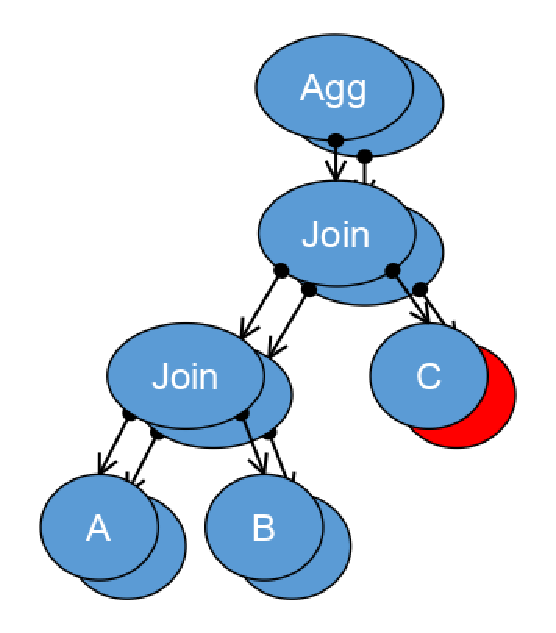
\includegraphics[scale=0.5]{compare_trees}
  \end{center}
\end{column}\end{columns}
% As a positive outcome here: you don't depend on syntax, tabulations and even (sometimes) names of the objects. You compare parse trees with oids in the leaf nodes.
% Negative outcome is tree comparison procedure. As much details it will check as much queries you can execute with the frozen plan.
% Short example. Right now we use core function equal() to compare parse trees. It gives us portability and responsibility. But if you change any aliases of any column or a table, the extension wouldn't find frozen plan for such a query. So, here is a room for improvements.
\end{frame}

\begin{frame}[fragile]\frametitle{Lesson 3}
\begin{columns}\begin{column}{0.5\textwidth}
To make overhead admissible, we should have kind of parse tree signature - queryId
\end{column}\begin{column}{0.5\textwidth}
  \begin{center}
    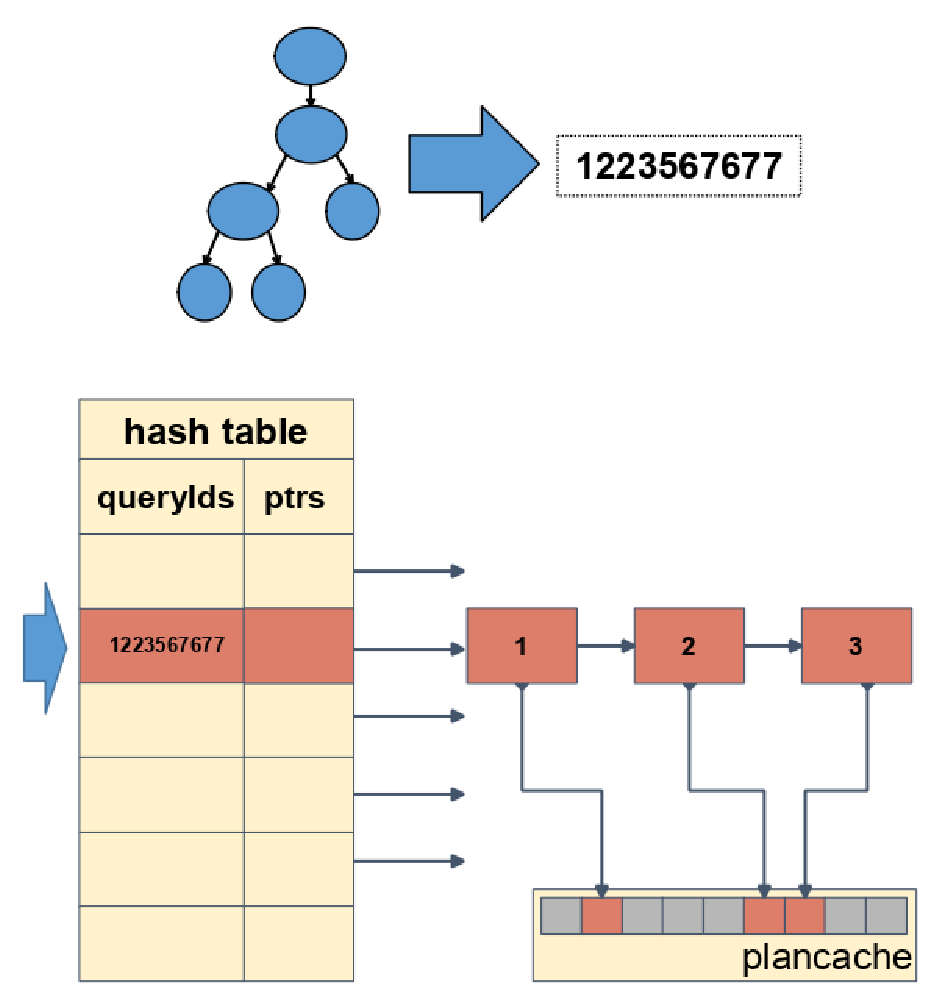
\includegraphics[scale=0.35]{queryid}
  \end{center}
\end{column}\end{columns}
\end{frame}

\begin{frame}[fragile]\frametitle{Lesson 4}
\begin{columns}\begin{column}{0.5\textwidth}
To apply plan freezing for parameterized queries we should '\textit{generalize}' the parse tree
\end{column}\begin{column}{0.5\textwidth}
  \begin{center}
    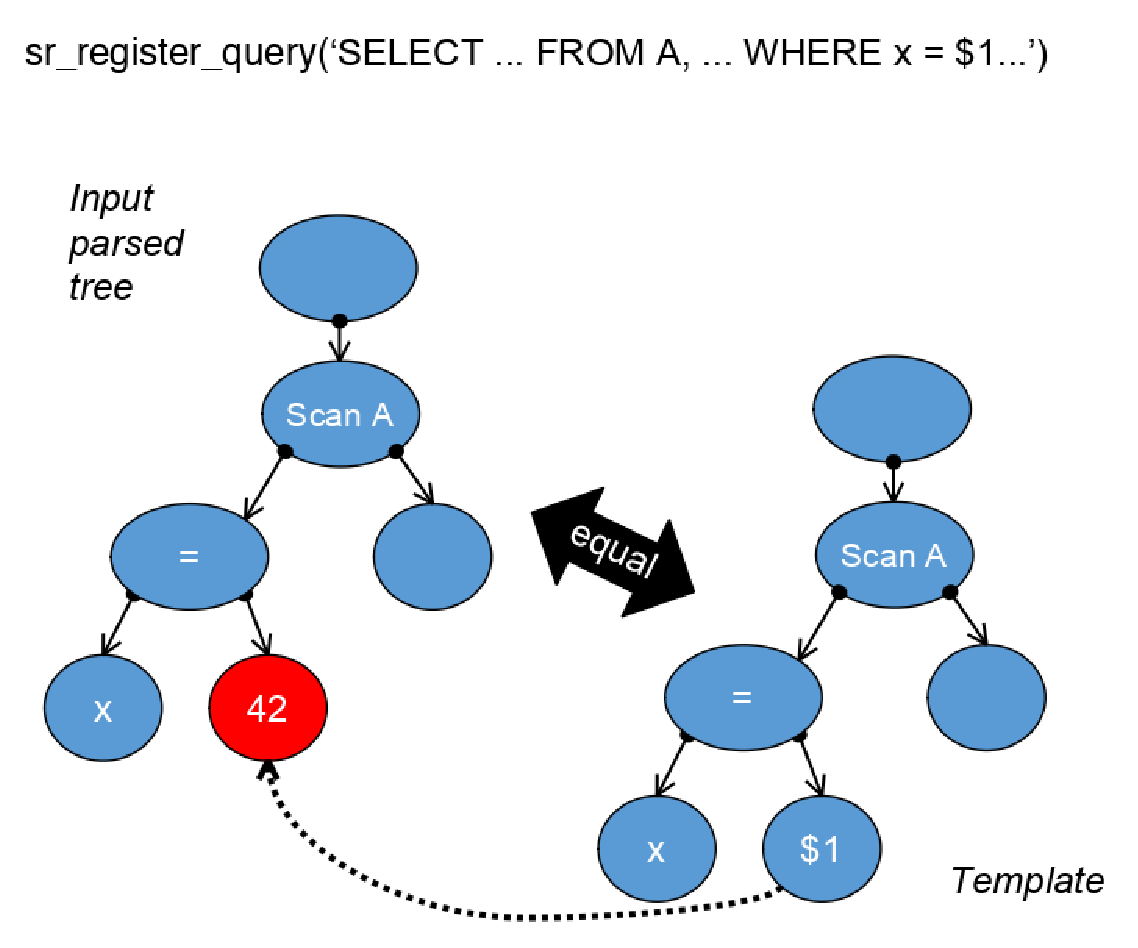
\includegraphics[scale=0.3]{tree_template}
  \end{center}
\end{column}\end{columns}
\end{frame}

\begin{frame}[fragile]\frametitle{Lesson 5}
\begin{columns}\begin{column}{0.4\textwidth}
The extension loading order matters
\end{column}\begin{column}{0.6\textwidth}
  \begin{center}
    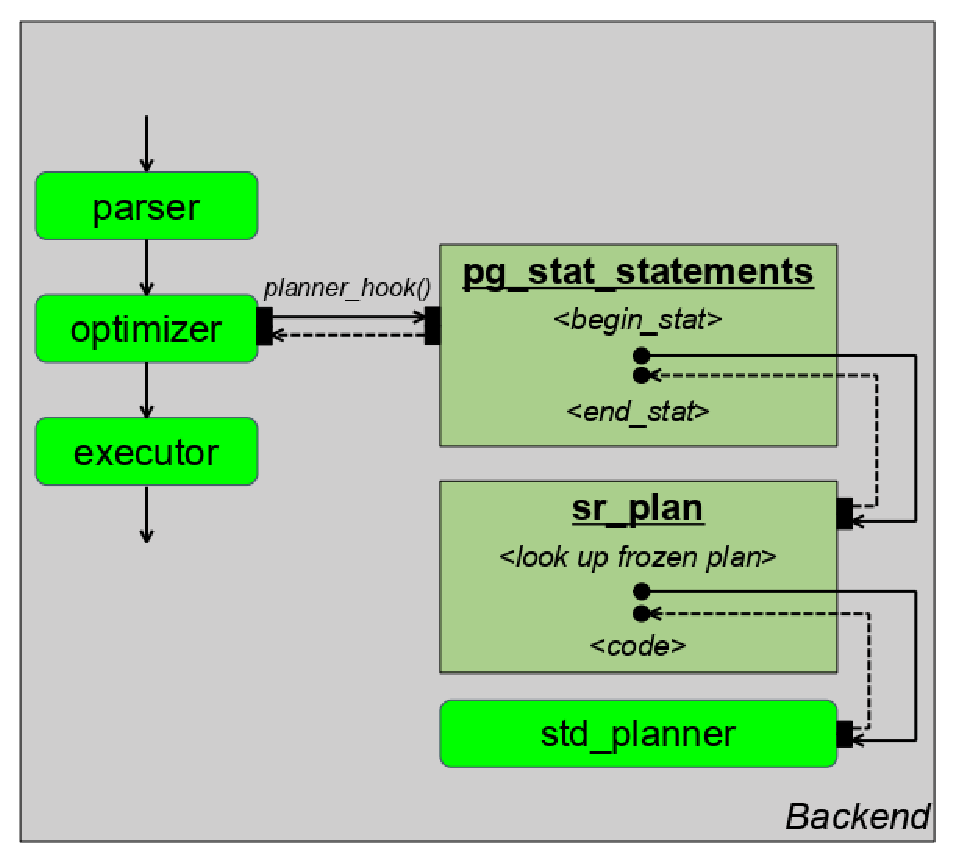
\includegraphics[scale=0.41]{hook_order}
  \end{center}
\end{column}\end{columns}
% Queue of hooks and how to avoid planning on frozen statements
\end{frame}

\begin{frame}[fragile]\frametitle{Points of overhead}
\begin{columns}\begin{column}{0.5\textwidth}
\begin{itemize}
  \item Parse tree comparison
  \item Plan invalidation
  \begin{itemize}
    \item Per-backend cache invalidation
    \item Disc storage sync
    \item Transactional issues
  \end{itemize}
\end{itemize}
\end{column}\begin{column}{0.5\textwidth}
  \begin{center}
    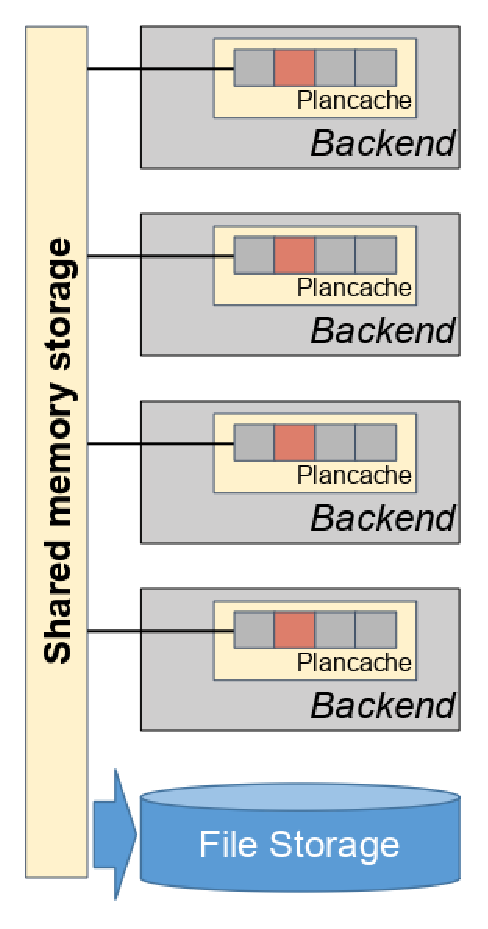
\includegraphics[scale=0.4]{plancache_invalidation}
  \end{center}
\end{column}\end{columns}
% Queue of hooks and how to avoid planning on frozen statements
\end{frame}

\begin{frame}[fragile]\frametitle{The future}
\begin{itemize}
  \item Detect bad plan and try something different
  \item Plan transfer procedure
  \item Global prepared statements
% Let me tell a bit about the future of this extension.
% It is made as an enterprise solution occasionally. We have been looking at this extension as a playground for much more interesting Core and EE features.
% GPS - it looks like we can move stored plan from shmem to the system catalog, to make it happens. Here is, of course, a lot of work with plan invalidation issues. But still, it is a good tool.
% The method of plan usage proof can be used for safe transfer to another instance with the BKI. Using subtransactions we can imagine such external tool for dump/restore of plans.
\end{itemize}
\end{frame}

\begin{frame}
\begin{center}
\begin{center}

\includegraphics[scale=0.1]{project_logo}
\end{center}
\huge{Questions ?}
\end{center}
\end{frame}

\end{document}
